%----------------------------------------------------------------------
\begin{frame}
   \frametitle{Example: Renal failure data from Steno}
{\small
Hovind P, Tarnow L, Rossing P, Carstensen B, and Parving H-H:
 Improved survival in patients obtaining remission of nephrotic range
  albuminuria in diabetic nephropathy.
  {\em Kidney Int.}, 66(3):1180--1186, 2004.}
\pause
\begin{itemize}[<+->]
\item Endpoint of interest: Death or end stage renal disease (ESRD),
  i.e. dialysis or kidney transplant.

\item 96 patients entering at nephrotic range albuminuria (NRA),
  i.e. U-alb$>300$mg/day.

\item Is remission from this condition (i.e return to
  U-alb$<300$mg/day) predictive of the prognosis?
\end{itemize}
\end{frame}

%----------------------------------------------------------------------
\begin{frame}

\small
\renewcommand{\arraystretch}{0.8}
\begin{tabular}{rlrrr}
\toprule
& & & \multicolumn{2}{r}{Remission} \\
\cmidrule{4-5}
& & Total & Yes & No \\
   \midrule
\multicolumn{2}{r}{No. patients          } &  125   &  32   &  93   \\
\multicolumn{2}{r}{No. events            } &   77   &   8   &  69   \\
\multicolumn{2}{r}{Follow-up time (years)} & 1084.7 & 259.9 & 824.8 \\
 \midrule
 \multicolumn{2}{l}{Cox-model:} \\
Timescale: & \multicolumn{4}{l}{Time since nephrotic range albuminuria
                       (NRA)} \\
    Entry: & \multicolumn{4}{l}{2.5 years of GFR-measurements after NRA} \\
  Outcome: & \multicolumn{4}{l}{ESRD or Death} \\
\multicolumn{2}{l}{Estimates:}
  & RR & 95\% c.i. & $\p$ \\
 \midrule
\multicolumn{2}{r}{Fixed covariates:} \\
\multicolumn{2}{r}{Sex (F vs. M):}             & 0.92 & (0.53,1.57) & 0.740 \\
\multicolumn{2}{r}{Age at NRA (per 10 years):} & 1.42 & (1.08,1.87) & 0.011 \\
 \\
\multicolumn{2}{r}{Time-dependent covariate:} \\
\multicolumn{2}{r}{Obtained remission:      }  & 0.28 & (0.13,0.59) & 0.001 \\
 \bottomrule
\end{tabular}
\renewcommand{\arraystretch}{1.0}
\normalsize
\end{frame}

%----------------------------------------------------------------------
\begin{frame}
% \includegraphics[height=\textheight]{c:/Bendix/Steno/PHov/nefro/graph/Nefro}
% \includegraphics[height=\textheight]{c:/Bendix/Steno/PHov/nefro/graph/Nefro-0}
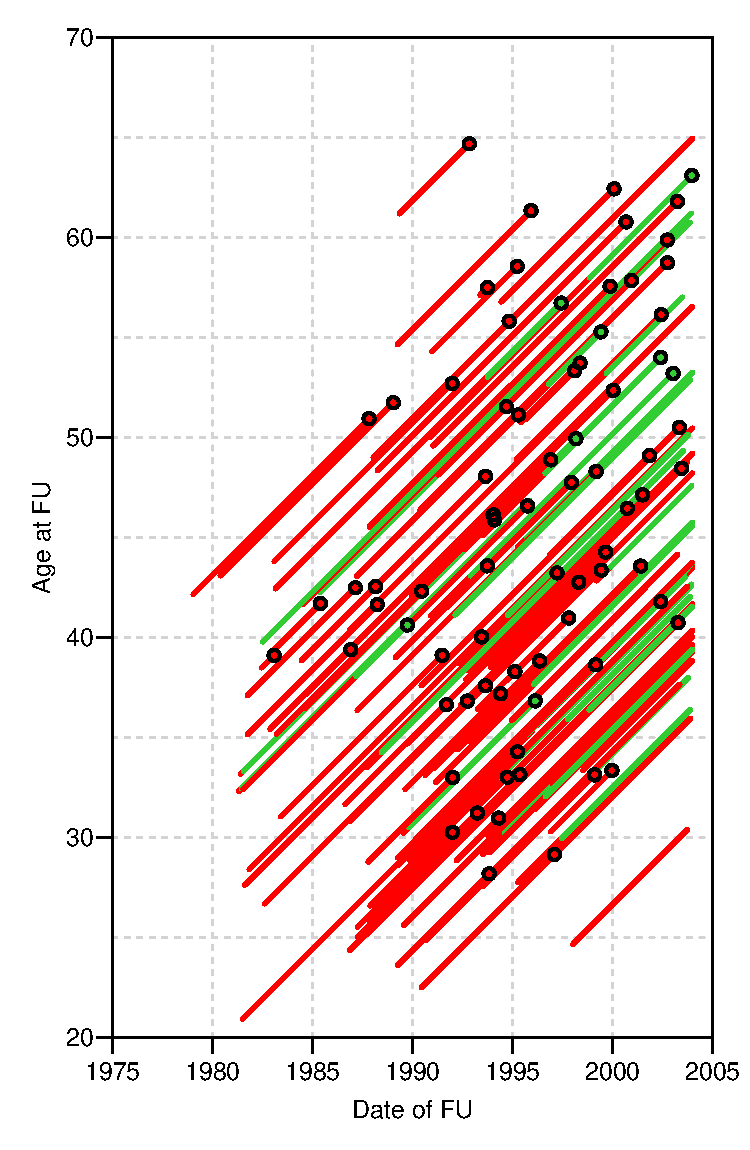
\includegraphics[height=\textheight,keepaspectratio]{./Ren-Lexis}
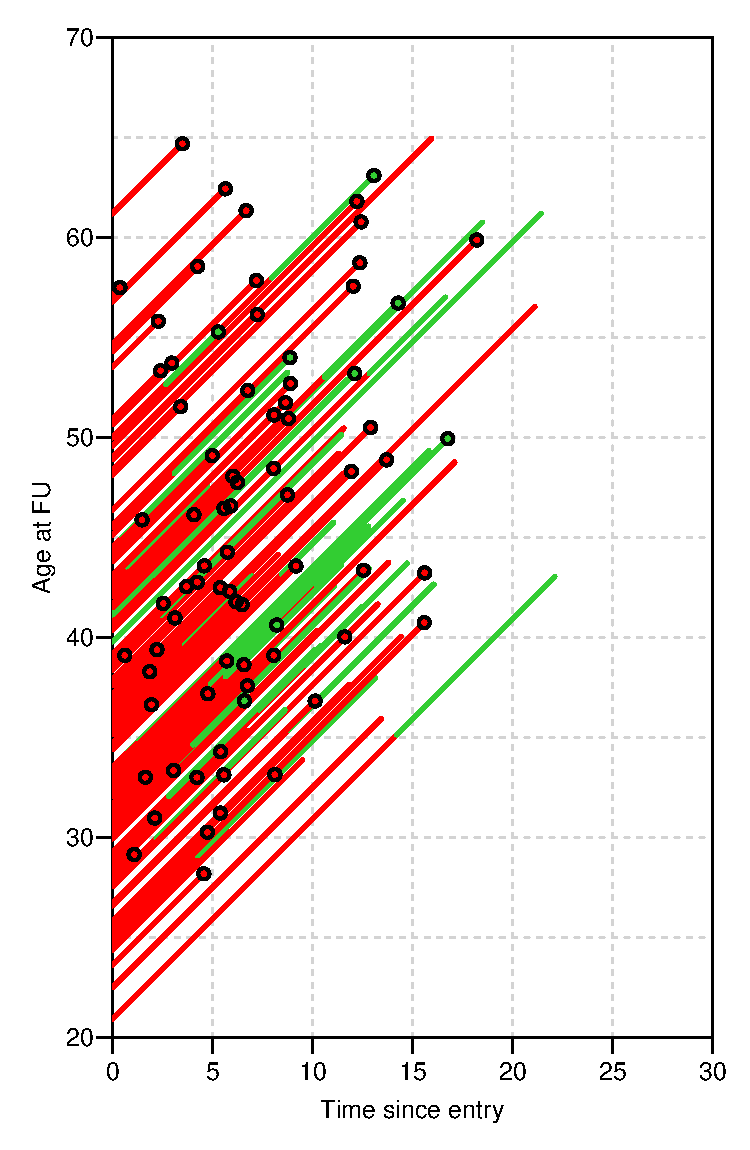
\includegraphics[height=\textheight,keepaspectratio]{./Ren-Lexis0}
\end{frame}

%----------------------------------------------------------------------
\begin{frame}[fragile]
   \frametitle{Features of the analysis}
\begin{itemize}
\item Remission is included as a time-dependent variable.
\item Age at entry is included as a fixed variable.
\end{itemize}
\small
\renewcommand{\baselinestretch}{0.9}
\begin{verbatim}
renal[1:5,]
id      dob      doe      dor      dox event
17 1967.944 1996.013       NA 1997.094     2
26 1959.306 1989.535 1989.814 1996.136     1
27 1962.014 1987.846       NA 1993.239     3
33 1950.747 1995.243 1995.717 2003.993     0
42 1961.296 1987.884 1996.650 2003.955     0
\end{verbatim}
\renewcommand{\baselinestretch}{1.0}
\normalsize
Note patient 26, 33 and 42 obtain remission.
\end{frame}

%----------------------------------------------------------------------
\begin{frame}[fragile]
\renewcommand{\baselinestretch}{0.8}
\footnotesize
\begin{verbatim}
> Lr <- Lexis(entry = list(per = doe,
+                          age = doe-dob,
+                          tfi = 0),
+              exit = list(per = dox),
+       exit.status = event>0,
+            states = c("NRA", "ESRD"),
+              data = renal)
> summary(Lr)

Transitions:
     To
From  NRA ESRD  Records:  Events: Risk time:  Persons:
  NRA  48   77       125       77    1084.67       125
\end{verbatim}
\normalsize
\renewcommand{\baselinestretch}{1.0}
\end{frame}

%----------------------------------------------------------------------
\begin{frame}[fragile]
\renewcommand{\baselinestretch}{0.8}
\footnotesize
\begin{verbatim}
> boxes(Lr, boxpos = list(x = c(25, 75),
+                         y = c(75, 25)),
+           scale.R = 100, show.BE = TRUE )
\end{verbatim}
\normalsize
\renewcommand{\baselinestretch}{1.0}
\begin{center}
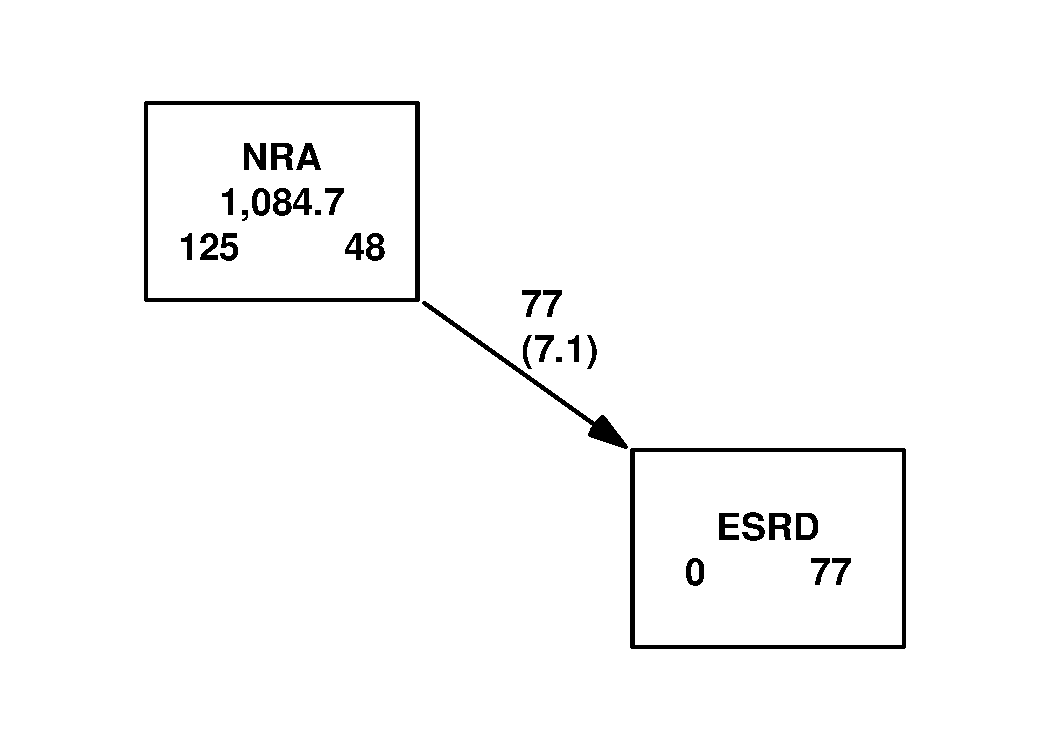
\includegraphics[height=0.7\textheight,keepaspectratio]{./NRA-mort}
\end{center}
\end{frame}

% %----------------------------------------------------------------------
% \begin{frame}{Illness-death model}
% \begin{center}
% 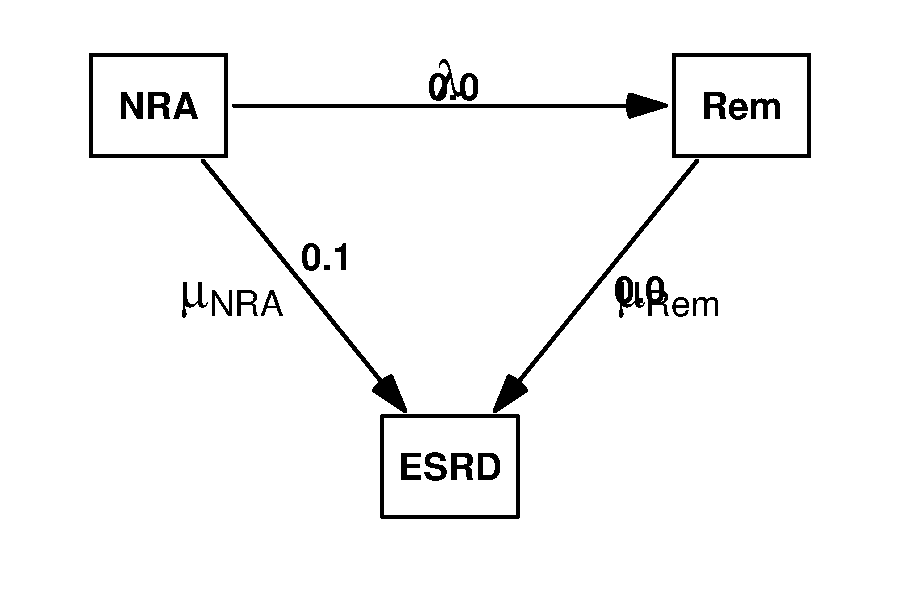
\includegraphics[height=0.6\textheight,keepaspectratio]{./NRA-death-par3}
% \end{center}
% \vspace*{-2em}
% \begin{tabular}{rl}
% $\lambda$: & remission rate.\\
% $\mu_\text{NRA}$: & mortality/ESRD rate \textbf{before} remission.\\
% $\mu_\text{rem}$: & mortality/ESRD rate \textbf{after} remission.
% \end{tabular}
% \end{frame}

%----------------------------------------------------------------------
\begin{frame}[fragile]{Cutting follow-up at remission: \texttt{cutLexis}}
\renewcommand{\baselinestretch}{0.8}
\footnotesize
\begin{verbatim}
> Lc <- cutLexis(Lr, cut = Lr$dor,
+                timescale = "per",
+                new.state = "Rem")
> summary(Lc)

Transitions:
     To
From  NRA Rem ESRD  Records:  Events: Risk time:  Persons:
  NRA  24  29   69       122       98     824.77       122
  Rem   0  24    8        32        8     259.90        32
  Sum  24  53   77       154      106    1084.67       125
\end{verbatim}
\normalsize
\renewcommand{\baselinestretch}{1.0}
\end{frame}

%----------------------------------------------------------------------
\begin{frame}[fragile]{Showing states and FU: \texttt{boxes.Lexis}}
\renewcommand{\baselinestretch}{0.8}
\footnotesize
\begin{verbatim}
> boxes(Lc, boxpos = list(x = c(15, 85, 50),
+                         y = c(85, 85, 20)),
+           scale.R = 100, show.BE = TRUE)
\end{verbatim}
\normalsize
\renewcommand{\baselinestretch}{1.0}
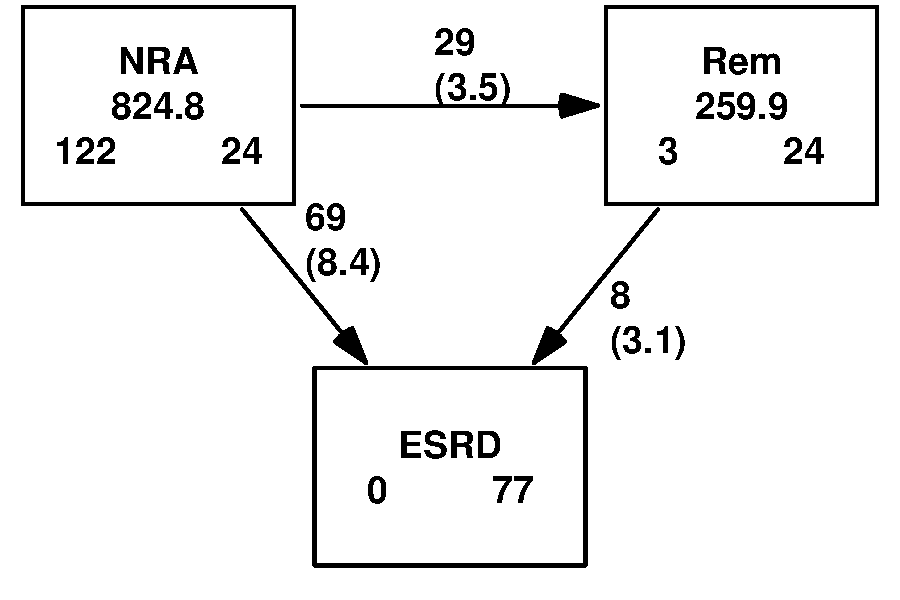
\includegraphics[height=0.6\textheight,keepaspectratio]{./NRA-death-3}
\end{frame}

%----------------------------------------------------------------------
\begin{frame}[fragile]{Cutting follow up at events: \texttt{cutLexis}}
\renewcommand{\baselinestretch}{0.8}
\footnotesize
\begin{semiverbatim}
> Lc <- cutLexis( Lr, cut = Lr$dor,
+               timescale = "per",
+               new.state = "Rem",
+            \alert<2->{split.states = TRUE})
> summary( Lc )

Transitions:
     To
From  NRA Rem ESRD\alert<3>{ ESRD(Rem)}  Records:  Events: Risk time:  Persons:
  NRA  24  29   69\alert<3>{         0}       122       98     824.77       122
  Rem   0  24    0\alert<3>{         8}        32        8     259.90        32
  Sum  24  53   69\alert<3>{         8}       154      106    1084.67       125
\end{semiverbatim} %$
\normalsize
\renewcommand{\baselinestretch}{1.0}
\end{frame}

%----------------------------------------------------------------------
\begin{frame}[fragile]{Showing states and FU: \texttt{boxes.Lexis}}
\renewcommand{\baselinestretch}{0.8}
\footnotesize
\begin{verbatim}
> boxes(Lc, boxpos = list(x = c(15, 85, 15, 85),
+                         y = c(85, 85, 20, 20)), 
+          scale.R = 100)
\end{verbatim}
\normalsize
\renewcommand{\baselinestretch}{1.0}
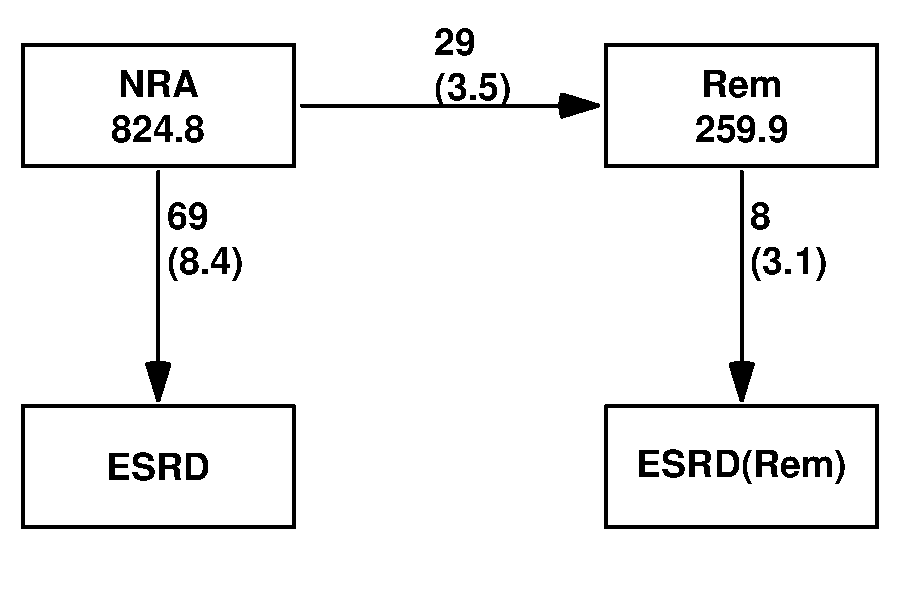
\includegraphics[height=0.7\textheight,keepaspectratio]{./NRA-death-4}
\end{frame}

%----------------------------------------------------------------------
\begin{frame}[fragile]{Likelihood for a general MS-model}
  \begin{itemize}[<+->]
  \item Product of likelihoods for each transition\\
        --- each one as for a survival model
  \item \textbf{Risk time} is the risk time in the ``From'' state
  \item \textbf{Events} are transitions to the ``To'' state
  \item All other transitions out of ``From'' are treated as \textbf{censorings}
  \item Possible to fit models

    \begin{itemize}
    \item separately for each transition
    \item jointly for transitions from \textbf{different} states
    \item jointly for different transitions out of the \textbf{same}
      state: \textbf{don't!}  
    \end{itemize}
    
  \end{itemize}
\end{frame}

% %----------------------------------------------------------------------
% \begin{frame}
% \ \\[-3ex]
% 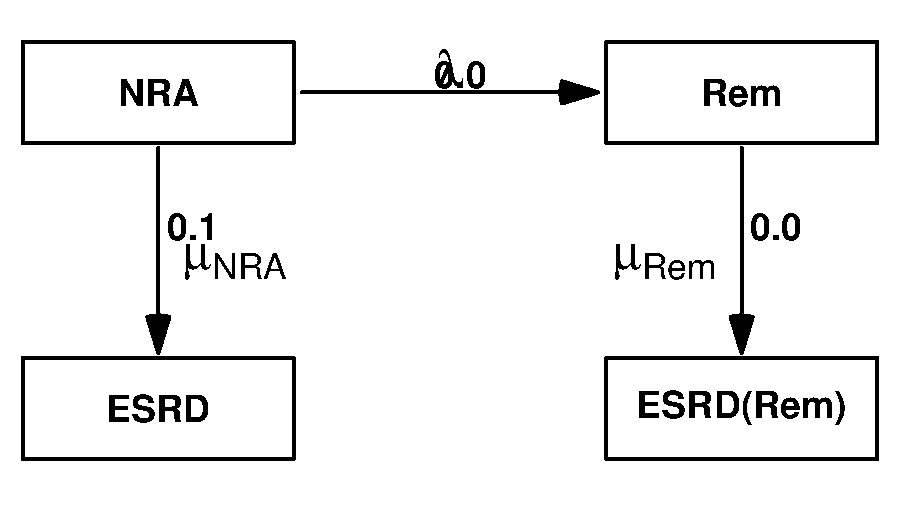
\includegraphics[height=0.55\textheight,keepaspectratio]{NRA-death-par4}
% \ \\[-1ex]
% Cox-analysis with remission as time-dependent covariate:
% \begin{itemize}[<+->]
% \item Ignores $\lambda$, the remission rate.
% \item Assumes $\mu_\text{NRA}$ and $\mu_\text{rem}$ use the same timescale.
% \end{itemize}
% \end{frame}

% %----------------------------------------------------------------------
% \begin{frame}{Model for all transitions}
% \begin{minipage}[b]{0.49\textwidth}
% \raggedright
% 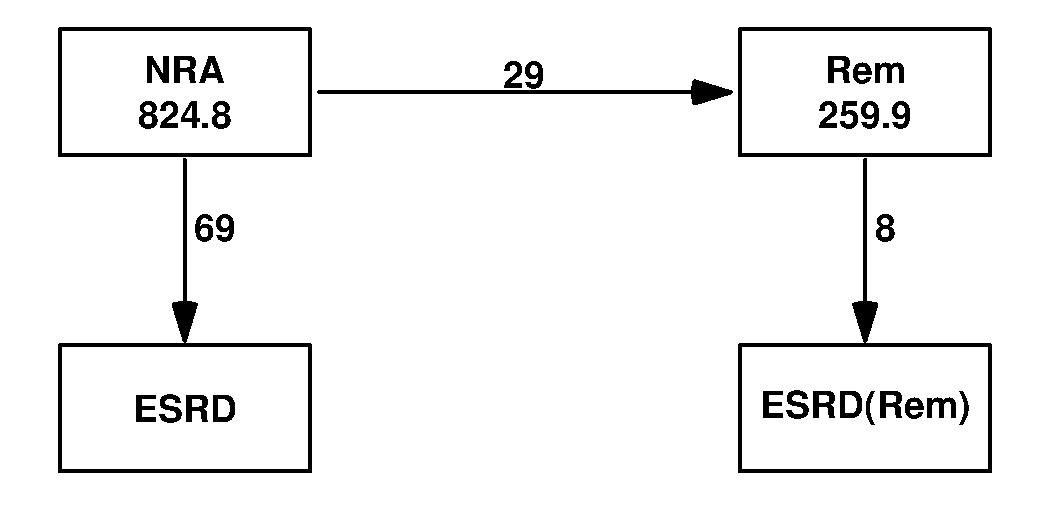
\includegraphics[width=\textwidth,keepaspectratio]{NRA-death-ann}\\
% \textbf{Cox-model:}
% \begin{itemize}
% \item Different timescales for transitions possible
% \item \ldots only one per transition
% \item No explicit representation of estimated rates.
% \end{itemize}
% \end{minipage}
% \hfill
% \begin{minipage}[b]{0.49\textwidth}
% \raggedright
% \textbf{Poisson-model:}
% \begin{itemize}
% \item Timescales can be different
% \item Multiple timescales can be accomodated simultaneously
% \item Explicit representation of all transition rates
% \end{itemize}
% \end{minipage}
% \end{frame}

%----------------------------------------------------------------------
\begin{frame}{Calculating state probabilities}
\ \\[-3em]
\begin{eqnarray*}
 \lefteqn{ \ptxt{Remission \textbf{before} time $t$} } \\ & = &
 \int_0^t \lambda(u) \exp\left( -\!\! \int_0^u \lambda(s) + \mu_\text{NRA}(s) \dif s
          \right) \dif u\\[1em]
 \lefteqn{ \ptxt{Being in remission \textbf{at} time $t$} } \\ & = &
 \int_0^t \lambda(u) \exp\left( -\!\! \int_0^u \lambda(s) +
                                               \mu_\text{NRA}(s) \dif s \right)
                     \times \\ & & \hspace*{8em}
                     \exp\left( -\!\! \int_u^t \mu_\text{rem}(s) \dif s \right)
          \dif u
\end{eqnarray*}
Note $\mu_\text{rem}$ could also depend on $u$, time since obtained remission.
\end{frame}

%----------------------------------------------------------------------
\begin{frame}[fragile]
  Sketch of programming, assuming that 
$\lambda$ (\texttt{lambda}), 
$\mu_\text{NRA}$ (\texttt{mu.nra}) and
$\mu_\text{rem}$ (\texttt{mu.rem}) are known at any age (stored in vectors)
\renewcommand{\baselinestretch}{0.85}
\footnotesize
\begin{verbatim}
c.rem      <- cumsum(lambda)
c.mort.nra <- cumsum(mu.nra)
c.mort.rem <- cumsum(mu.rem)
pr1 <- cumsum(lambda * exp(-(c.rem + c.mort.nra)))

intgr(t,s) <- 
function(t,s){
lambda[s] * exp(-(c.rem[s] + c.mort.nra[s])) *
            exp(-(c.mort.rem[t] - c.mort.rem[s]))
             }
for(t in 1:100) p2[t] <- sum(intgr(t,1:t))
\end{verbatim}
\normalsize
\renewcommand{\baselinestretch}{1.00}
If $\mu_\text{rem}$ also depends on time since remission, then
\texttt{c.mort.rem} should have an extra argument---technically very complicated
\end{frame}

% %----------------------------------------------------------------------
% \begin{frame}
%    \frametitle{Calculation of state probabilities}
% The possibility of computing the state-occupancy probabilities relies
% on:
%    \begin{itemize}[<+->]
%    \item Availablity of closed-form formulae for the probailities
%      in terms of the transition rates
%    \item Transition rates are assumed to be continuous functions of time
%    \item Transition rates can be calulated at any point of time\ldots
%    \item This will allow simple calulation of the integrals from the
%      closed-form expressions.
%    \end{itemize}
% \end{frame}
